\documentclass[12pt]{book}

\usepackage[utf8]{inputenc}
\usepackage[T1]{fontenc}
\usepackage{geometry}
\usepackage{graphicx}
\usepackage[spanish]{babel}
\usepackage{amsthm}
\usepackage{amsmath}
\usepackage{calrsfs}
\usepackage{trfsigns}

\newtheorem{thm}{Teorema}[section]
\theoremstyle{definition}
\newtheorem{dfn}{Definición}[section]
\theoremstyle{remark}
\newtheorem{note}{Nota}[section]
\theoremstyle{plain}
\newtheorem{lem}[thm]{Lema}

\geometry{letterpaper}

\title{Simulación por Elementos Finitos}
\author{Dr. Casimiro Gómez González\\
	Facultad de Electrónica, UPAEP\\
               correo: casimiro.gomez@upaep.mx\\
               Tel: 222 229 9428}
\date{Otoño 2011}

\begin{document}
\frontmatter
\maketitle

\chapter{Prólogo}

El presente manual es para el diseño y simulación de software por elementos finitos tanto mecánico como fluidos. Utilizando Code Aster y Code Saturne. 
Tambien se utiliza Salome Meca para el preprocesamiento y post procesamiento.

\begin{flushright}

El autor\\
Casimiro Gómez González\\
Doctor en Ingeniería Mecatrónica
\end{flushright}

\tableofcontents

\mainmatter
\chapter{Introducción}
Code\_Aster puede realizar cálculos estructurales de los fenómenos térmicos, 
cálculos mecánicos, acústicos termo-mecánica y termo-hidro-mecánico, junto con 
un comportamiento lineal o no lineal y los cálculos de acústica interior.

Las no linealidades están en el comportamiento de los materiales 
(plasticidad, viscoplasticidad, daño, los efectos metalúrgicos, hidratación y 
secado del hormigón, ...), grandes deformaciones y rotaciones grandes y el 
contacto con la fricción. Consulte el folleto de presentación Code\_Aster para 
la presentación de diferentes características.

Los estudios actuales de la industria requieren la aplicación de herramientas para la 
creación de redes y gráficos, que no forman parte del código. Sin embargo, 
hay varias herramientas utilizadas para estas operaciones a través de la interfaz 
de los procedimientos incorporados en el código.

Para llevar a cabo un estudio, el usuario general deberá preparar dos archivos de datos:

\begin{itemize}
 \item el archivo de malla:
Este archivo define la descripción geométrica y topológica de la malla sin elegir 
en esta fase, el tipo de formulación de elementos finitos utilizado o el fenómeno 
físico que está siendo modelado. Algunos estudios pueden llevar al uso de múltiples
 archivos de malla.
Este archivo de malla es generalmente producido por los comandos integrados para 
Code\_Aster a partir de un archivo proveniente de un software de mallado 
utilizado en el pre-procesador (SALOMÉ Gibi, gmsh, IDEAS ...).

La información que debe contener este archivo son específicos de Code\_Aster. Ellos 
definen entidades clásicas de los métodos de elementos finitos:
\begin{itemize}
 \item nodos: los puntos se define por su nombre y por sus coordenadas cartesianas en
2D o 3D.
 \item Mallas: Las figuras topológicas llamadas planas o volumen 
(punto, segmento, triángulo, cuadrángulo, tetraedro, ...) que pueden ser aplicados
 en diferentes tipos de elementos finitos, las condiciones de contorno o cargas.
\end{itemize}
Para mejorar la seguridad y comodidad de uso de operaciones de modelado y 
procesamiento de los resultados, podemos definir en el archivo de malla, los 
niveles más altos de las entidades,que tienen alguna propiedad en común y que pueden 
ser utilizados directamente por su nombre:

\begin{itemize}
 \item Grupos de Nodos: listas llamadas de nombres de los nodos
 \item Grupos de malla: las listas llamada de nombres de mallas
\end{itemize}
Tenga en cuenta, ahora que todas las entidades geométricas manipuladas (nodos,
mallas, grupos de nodos y grupos de mallas) son nombrados por el usuario y disponibles 
en todo momento por su nombre (8 carácteres máximo).El usuario puede utilizar esta
 oportunidad para identificar explícitamente ciertas partes de la estructura 
estudiada y facilitar así la tabulación de los resultados. La numeración de las entidades 
no se explica: sólo sirve para señalar a los valores internos de las diferentes variables 
involucradas.
 \item el archivo de comandos:para definir el texto del comando que permite:
\begin{itemize}
 \item Leer y, posiblemente, mejorar el fichero de datos de la malla (u otras fuentes de 
resultados externos)
 \item afectar el modelado de datos en las entidades de la malla
 \item  cadena de operaciones de tratamiento diferentes:cálculos, tratamientos específicos posteriores,
 \item publicar los resultados en archivos diferentes.
\end{itemize}

Cet exemple peut être celui des travaux pratiques de la formation ‘Initiation au Code de mécanique : Code_Aster’ qui correspond au cas-test FORMA01 : •L’énoncé est disponible sur le site de Code_Aster page exemple/cas-test de validation. •Les fichiers d’entrée sont disponibles sur le serveur de calcul aster sous /aster/v7/STA7/astest : ➔le fichier de commande (forma01f.comm), ➔le fichier de maillage (forma01f.mgib). •Les fichiers de sortie sont : ➔le fichier de résultats (tuyau.resu), ➔le fichier de message (tuyau.mess). Cet exemple passe avec une mémoire de 64 Mo et un temps de 60s. Si vous rencontrez un problème lors de cette étape, nous vous proposons de vérifier les points suivants : •le bouton ETUDE doit être coché, •la machine d’exécution est clayastr, •l’option --check d’astk permet de vérifier les fichiers .rhosts (cf. [U1.04.00]) sur le serveur de fichiers et sur le serveur de calcul aster. L’utilisateur doit disposer d’un compte sur un serveur de fichiers et d’un compte sur le serveur de calcul aster. •la configuration astk est correcte. Vérifiez auprès de votre correspondant local.
Quizás quisiste decir: ou d'autres sources de résultats externes
Escribe texto o la dirección de un sitio web, o bien, traduce un documento.
Cancelar
Escuchar
Leer fonéticamente
traducción del francés al español
El texto del comando hace referencia a los nombres de las entidades geométricas definidas en el 
archivo de malla.
\end{itemize}


\chapter{Introducción a Code Aster}

\section{Como Empezar Code\_Aster, tomado del U0.00.01}
Code\_Aster es un código general para el estudio del comportamiento mecánico de 
las estructuras.
Para entender Code\_Aster, se recomienda:
\begin{itemize}
 \item Consulta de la documentación
 \item Uso de la interfaz gráfica de usuario astk Code\_Aster un ejemplo sencillo,
 \item El uso de EFICAS para desarrollar su archivo de control
\end{itemize}


Se recomiendan los tres puntos como la guía esencial para estudiar.
\section{Documentación}

El sitio web (www.code-aster.org) dedicado a  Code\_Aster es una fuente de información.
Para entender Code\_Aster, consulte la página de Uso/Introducción:
\begin{itemize}
 \item Usted puede consultar la documentación general a: 
     \begin{itemize}
       \item Introducción a Code\_Aster [U1.02.00] 
       \item  Los principios básicos de la utilización de Code\_Aster [U1.03.00]. 
     \end{itemize}
 \item Usted puede confiar en ejemplos sencillos para familiarizarse con el uso 
de Code\_Aster.
\end{itemize}

Para llevar a cabo su estudio, se puede ver:

\begin{itemize}
 \item  En la documentación [U1.04.00], la interfaz de acceso a 
Code\_Aster: astk.
 \item Todos los casos de prueba de un modelo básico.
\end{itemize}
A continuación, puede explorar más a fondo con los siguientes documentos:
\begin{itemize}
 \item Toda la documentación de uso.
 \item La página de capacitación que ofrece todas las diferentes presentaciones y 
sobre todo la capacitación ``Introducción a la Mecánica Código: Code\_Aster'' 
(para acceder a esta página, primero debe identificarse).
\end{itemize}

\subsection{Recomendación}

La primero es crear un inicio de sesión en el sitio de intranet 
Code\_Aster. Este se ofrece en todas las páginas del sitio.


\section{Interfaz gráfica astk}
astk es la interfaz gráfica que permite organizar los cálculos de Aster: preparar 
los datos, organizar los archivos, el acceso a las herramientas de pre\-y 
post\-procesamiento, lanzamiento y seguimiento de los cálculos. Su documentación 
está disponible en el sitio Code\_Aster [\verb|U1.04.00|].

Proponemos primero para familiarizarse con un ejemplo sencillo astk existente. Esto
 evitará que las dificultades asociadas a acumular astk y las de un nuevo estudio.

\section{El estudio del comportamiento mecánico de las estructuras}
Code\_Aster es un código general para el estudio del comportamiento mecánico
 de las estructuras.

El principal objetivo es la mecánica de sólidos deformables: lo que justifica 
el número de características unidos al fenómeno mecánico. Sin embargo, el estudio 
del comportamiento mecánico de los componentes industriales requiere de modelado
 ante el estrés que están sometidos, o los fenómenos físicos que modifican 
los parámetros de este comportamiento (fluido interno o externo, la temperatura, 
los esfuerzos de cambio de fase metalúrgica de origen electro-magnética ...). Por 
estas razones, Code\_Aster ofrece muchas posibilidades de ``encadenamiento'' de los 
fenómenos mecánicos con los fenómenos térmicos o acústicos, o con software externo,
 y se juntan en un problema ``kit`` de construcción termo-hidro-mecánica. Aunque 
Code\_Aster se puede utilizar para muchos problemas de análisis estructural 
(código general), se ha desarrollado especialmente para permitir el estudio de 
los componentes de los materiales o maquinaria utilizada en el campo de la 
generación y transmisión de electricidad. Así se dio prioridad a la modelización 
de estructuras metálicas geomateriales isotrópico y componentes estructurales de 
material de hormigón armado o compuesto.

El análisis no lineal, tantos Mecánicos como Térmicos, están en el corazón de 
Code\_Aster: para hacer un tratamiento eficaz se han hecho necesarios el 
desarrollo de algoritmos eficientes y relativamente sencillo de usar, incluso 
si el objetivo no es operar en ''recuadro negro''. Para estudios complejos, es 
necesario comprender la 
naturaleza de las operaciones realizadas por el código, para que puedas trabajar
 óptimamente es necesario referirse a los archivos que detallan los métodos y
 modelos teóricos, agrupados en el Manual de de referencia.

El aseguramiento de la calidad para el desarrollo de software y la implementación 
de estudios industriales justifica varias opciones:

Que existan códigos de una versión de referencia fijo y documentado, el suministro
 de algoritmos completos, pero en principio comandos fijos con parámetros de 
ortogonalidad (independencia del contexto de uso), la meta de realización de 
modelos utilizables.

Un análisis estructural se lleva a cabo con Code\_Aster en la secuencia de una 
serie de comandos que se describen en un ``archivo de comandos`` en formato de 
texto. El motor y el intérprete del archivo de comandos es el lenguaje de script
 PYTHON. Por tanto, es posible utilizar todas las características proporcionadas 
por Python. Véase especialmente la documentación [U1.03.01], [U1.03.02] y ejemplos
 de uso [U1.05.00] y [U1.05.01]. Cada orden (por ejemplo, la lectura de la malla, 
los datos del material condición, cálculo estático lineal) produjo un ``resultado 
de concepto'', todas las estructuras de datos que el usuario puede manipular y la 
reutilización de los pedidos posteriores del cálculo (por ejemplo, la creación 
de redes, el material de datos de campo, el campo de desplazamientos ...).

La sintaxis de todos los comandos se describen y analizan los libros de texto U4 y 
U7 documentación de uso.

Para simplificar la tarea del usuario, hay comandos globales que incluyen la
secuencia de las operaciones para un número de casos de cálculo (por ejemplo, 
lineal estática - comando MECA\_STATIQUE, no lineal estático - Comando 
STAT\_NON\_LINE,
no térmicos comando THER\_NON\_LINE , etc). Algunos se han desarrollado directamente 
en una forma integrada, los demás son macro-comandos de Python que sólo gestionan
las llamadas a la unidad de comandos diferentes (como MACRO\_MATR\_ASSE para calcular
 y ensamblar las matrices de masa, amortiguamiento y rigidez una estructura).
También hay controles macro, especialmente dedicado a las aplicaciones específicas 
(ver [§ 4]).



\chapter{Comandos de CODE\_ASTER}

Code Aster es un ``solver'' de elementos finitos:
\begin{itemize}
 \item sin herramientas sofisticadas para crear una geometría y para malla
 \item no hay imágenes post-procesamiento de colores
 \item Sin interfaces “click 'n' drop”
\end{itemize}

\begin{figure}
\centering
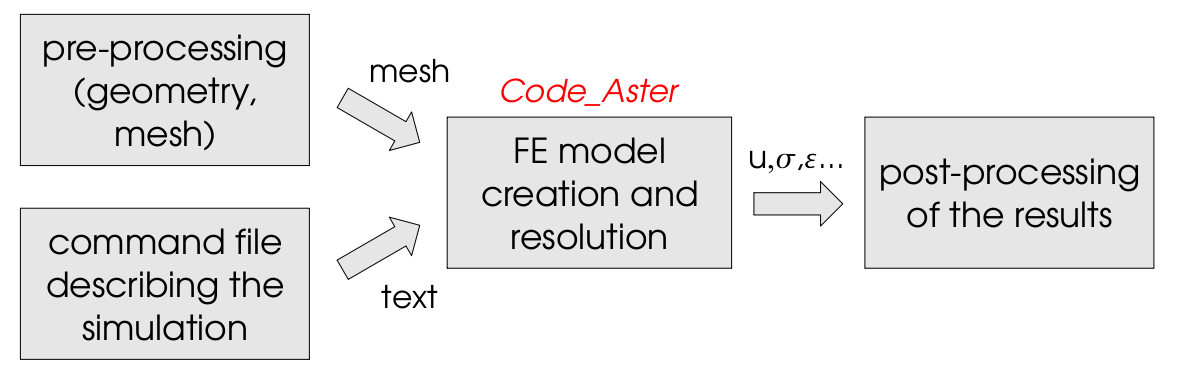
\includegraphics[width=5in]{Procesamiento.png}
\caption{Diseño y simulación por elementos finitos}
\label{fig1}
\end{figure}
Se muestra un diagrama a bloques de la simulación por elementos finitos, la
primera etapa esta formada por dos bloques: El preprocesamiento donde se
realiza el diseño en cad y la generación del mallado, y el archivo de
comandos, el cual describe las características de la simulación así como las
propiedades del modelo. En la segunda etapa se crea el modelo por elementos
finitos y se realiza la simulaci'on con Code Aster. Y como tercera y última
etapa se realizá el post procesamiento.

Varias herramientas pueden ser usadas para crear una malla y para 
visualizar resultados, en la medida que existe el módulo de importar/exportar 
en Code Aster:
\begin{itemize}
 \item Gmsh
 \item I-DEAS
 \item Gibi
 \item Cualquier herramienta capaz de importar/exportar mallas en formato MED
\end{itemize}

MED es un formato de plataforma independiente para el intercambio de datos de mallas
(nodos, elementos, grupos de nodos, grupos de elementos) y campos definidos en estos 
datos (e.g. estreses, tensión, desplazamientos, conjuntos de nivel...). Las 
librerías para manejar archivos MED estan disponibles libremente. 

\begin{figure}
\centering
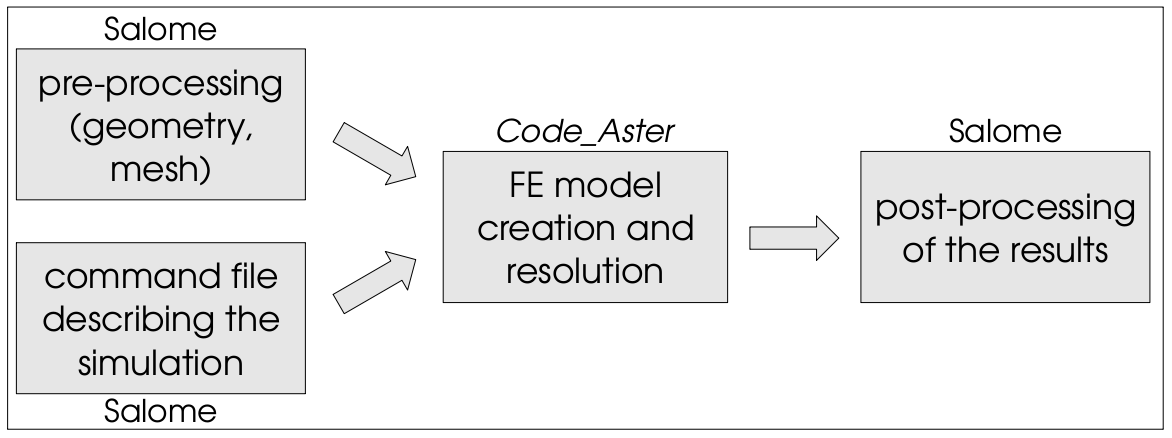
\includegraphics[width=5in]{SalomeMeca.png}
\caption{Arquitectura Salome Meca}
\label{fig2}
\end{figure}
Aún si Code Aster esta oculto atras de la interfaz gráfica de Salome-Meca, la manera 
en la cual Salome y Code Aster interectuan determina como el modelo por elementos
finitos es creado

\begin{figure}
\centering
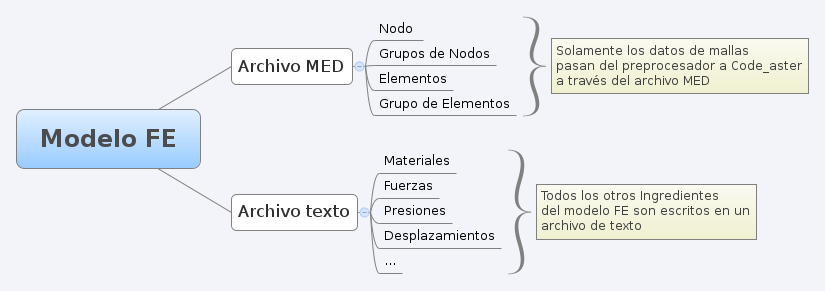
\includegraphics[width=5.5in]{ModeloFE.png}
\caption{Formatos de Salome Meca}
\label{fig3}
\end{figure}

Para que los datos introducidos en el ``wizard'' sean enlazados a la malla sean 
incluídas en el archivo MED, debes crear grupos de nodos, elementos, bordes y caras 
en la malla. Puedes definir estos grupos en la geometría del modelo o directamente 
en la malla. El usar los grupos de la geometría permite la modificación de la malla
si necesidad de redefinir los grupos. En el ``wizard'' puedes usar estos grupos para
aplicar las condiciones de frontera, fuerzas, presiones, materiales y demas.
Una vez Code aster ha resuelto el modelo FE, los resultados son importados en 
Salome-Meca a través de dos archivos de texto:

\begin{itemize}
 \item .mess: Contiene la salida de Code Aster para cada comando. Los errores y mensajes de advertencia son reportados en este archivo.
\item .resu contiene la salida de algunos resultados de Code Aster en forma de tabla.
\end{itemize}
Se pueden leer estos archivos directamente dentro de Salome-Meca.
La única manera para acceder a todas las características de Code Aster es manejar 
directamente el archivo de comandos a mano:

\begin{itemize}
 \item El archivo de comandos es un archivo de texto
 \item Una interfaz gráfica llamada Eficas puede ser usada para simplificar esta tarea.
\end{itemize}

Usando Eficas tu puedes:

\begin{itemize}
 \item Crea un archivo de comando sintacticamente correcto
 \item Crea un archivo de comando a mano sin recordar todas las opciones de cada comando
\end{itemize}

Sin embargo, se debe editar el archivo de comando a mano usando un editor
de texto si se quiere obtener mas del codigo de Code aster.
\begin{itemize}
 \item Usando las últimas características del software
 \item Usando programación Python
\end{itemize}

\section{Programas para Code Aster }

Los programas para code aster tienen una estructura definida y comandos definidos,
el lenguaje de base es python. Empezaremos definiendo los comandos en el orden 
en el que se recomienda deben aparecer.

\subsection{Comando DEBUT}

Esta función, \textbf{DEBUT()}, es usada para iniciar un nuevo análisis. Si este análisis es la 
continuación de uno previo, se debe utilizar la función \textbf{POURSUITE()}

\subsection{Comando DEFI\_MATERIAU}

El comando DEFI\_MATERIAU define las propiedades mecánicas de un material. Por ejemplo
si a una material llamado MA se le desea asignar sus propiedades elásticas se utiliza 
la palabra clave ELAS, de la siguiente forma

\begin{verbatim}
MA=DEFI_MATERIAU(ELAS=_F(E=210000000000.0,NU=0.3,),);
\end{verbatim}

Cada comando acepta uno o más parámetros identificados por una palabra clave:

\begin{verbatim}
 concepto = COMANDO(keyword_1=xxx,
                    keyword_2=yyy,
                    ...
                    keyword_n=zzz)
\end{verbatim}

En el caso de una palabra clave simple, su valor se proporciona directamente
despues del $=$. Esto puede ser un simple valor (ejemplo un entero, un valor real o
otro concepto) o una lista de valores simples:

\begin{verbatim}
 concepto_1 = COMANDO_1(simple_keyword_1=3)

 concepto_2 = COMANDO_2(simple_keyword_1=1.56,
                        simple_keyword_2=(1.0,0.0,5.6),
                        simple_keyword_3=concepto_1)
\end{verbatim}

En el caso de una palabra clave compuesta, sus valores son una lista de palabras claves
simples:

\begin{verbatim}
 concepto_1 = COMANDO_1(simple_keyword_1=3.0)

 concepto_2 = COMANDO_2(simple_keyword_1=1.56,
                       composed_keyword_1=_F(
                        simple_keyword_2=3.1415,
                        simple_keyword_3=concepto_1),)
\end{verbatim}

La lista de palabras claves simples de una palabra clave compuesta se da dentro de
\verb*|_F(...)|. La letra significa ``facteur'' en frances.


En el comando:

\begin{verbatim}
MA=DEFI_MATERIAU(ELAS=_F(E=210000000000.0,NU=0.3,),);
\end{verbatim}

La constante elástica es dada por la palabra clave ELAS, en donde el módulo de YOUNG
(E) y la razón de Poisson (NU) estan dentro de una palabra clave compuesta de
dos palabras claves simples. La definiciones del material estan dentro del concepto
llamado MA, el tamaño máximo de los conceptos es de 8 carácteres. Si el concepto
a utilizar existe antes de la ejecución del comando, se dispara un error y el análisis 
es abortado. 

Este concepto es un objeto de Python. Esto significa que tiene un tipo asociado:
\begin{itemize}
 \item El concepto resultado de MA es automaticamente creado por el comando, 
quien determina tambien el tipo
 \item El concepto MA puede ser usado como un valor de una palabra clave simple
solamente si sus tipos coinciden con el tipo requerido por la palabra clave.
\end{itemize}

Por ejemplo, si se desean definir dos materiales elásticos (un acero genérico y
un aluminio genérico). Estos dos materiales tienen diferentes valores del
módulo de Young pero el mismo (mas o menos) valor de la razón de Poisson. Para
forzar esta igualdad, se declara de la siguiente manera:
\begin{verbatim}
steel=DEFI_MATERIAU(ELAS=_F(E=2.06E11,
                         NU=0.3,),);
alu=DEFI_MATERIAU(ELAS=_F(E=0.76E11,
                         NU=steel,),);
\end{verbatim}

Esto es incorrecto debido a que \verb*|steel| es un concepto de tipo materiales
mientras que la palabra clave \verb*|NU| necesita un concepto de tipo real. La 
forma correcta de hacer esto, es usar una variable (no hay que olvidad que estamos
escribiendo en código python).

\begin{verbatim}
poisson=0.3
steel=DEFI_MATERIAU(ELAS=_F(E=2.06E11,
                         NU=poisson,),);
alu=DEFI_MATERIAU(ELAS=_F(E=0.76E11,
                         NU=poisson,),);
\end{verbatim}

\subsection{Comando LIRE\_MAILLAGE}
En Code Aster una malla es simplemente una lista de nodos (numeros y coordenadas)
y elementos (sus definiciones en términos de formas geométricas y definición 
de nodos). Todo estará contenido en el concepto MAIL. La malla esta contenida
en un archivo MED (\verb*|FORMAT='MED'|). Como en el caso de LIRE\_MAILLAGE, hay 
otros comandos que trabajan sobre archivos (de entrada o salida). El nombre
de los archivos para leer o escribir por un comando no es especificado en el archivos
de comandos pero fuera:
\begin{itemize}
 \item Esta abstracción facilita la creación de scripts, como en el caso estudios 
paramétricos donde el mismo análisis esta corriendo usando diferente mallas
 \item Es realmente práctico en todos los casos en los cuales uno o más de los 
archivos de entrada/salida cambia (diferentes nombres o paths, diferentes mallas...)
nada cambia en el archivo de comando.
\end{itemize}

Una herramienta gráfica \textbf{ASTK}, puede usado para listar todos los archivos 
necesarios para la simulación.
Si se utiliza Salome-Meca, los archivos de entrada/salida son automáticamente 
enlazadas a el archivo de comandos y no hay que hacer nada.

Esto es cierto en el caso en el cual se usa Salome-Meca para crear un archivo 
básico de comandos y entonces se puede usar Eficas para modificarlo.

Cada archivo tiene un \textbf{tipo} asociado:

\begin{figure}
\centering
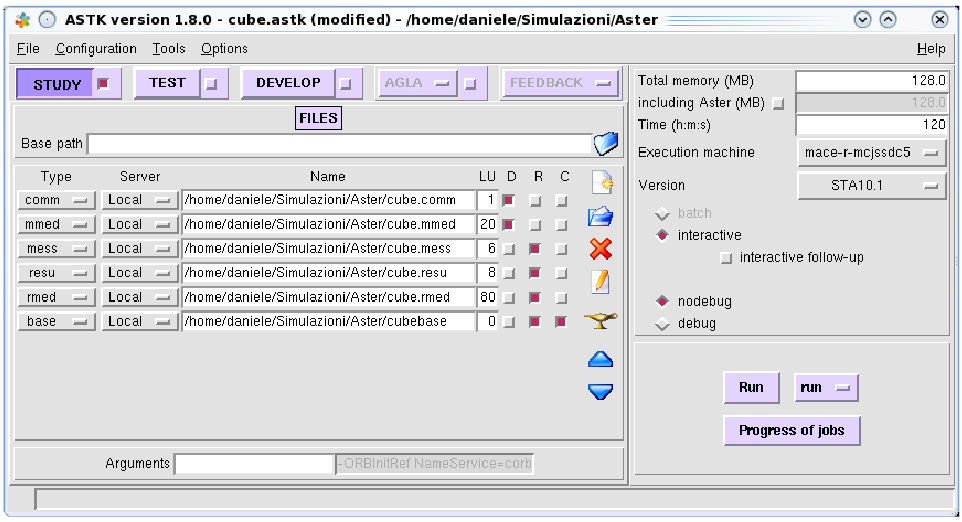
\includegraphics[width=5in]{tipos.png}
\caption{Tipos de archivos}
\label{fig4}
\end{figure}

Cada tipo tiene una \textbf{unidad lógica} numérica asociada. Cada comando accede
a un archivo (lectura/escritura) a través de su número de unidad lógica y no su nombre. 

Los archivos básicos manejados para cada simulación son:
\begin{itemize}
 \item comm: Es el archivo de comandos
 \item mmed: Es el archivo MED que contiene la malla.
 \item mess: Un archivo de texto que contiene la salida del ``solver'' (mensajes, errores,
y advertencias)
 \item resu Un archivo de texto que contiene los resultados de la 
simulación en formato de tabla
 \item rmed: Este es un archivo MED que contiene los resultados de la simlación
 \item base: Este es una carpeta que contiene la base de datos de salida del solver. Esta
será usada para continuar la simulación (en el caso de que se utilice el 
comando POURSUITE) o para post-procesamiento.
\end{itemize}

Cada uno de este tipo de archivos tiene un número lógico asigando por defecto (ver 
fig \ref{fig5}).

\begin{figure}
\centering
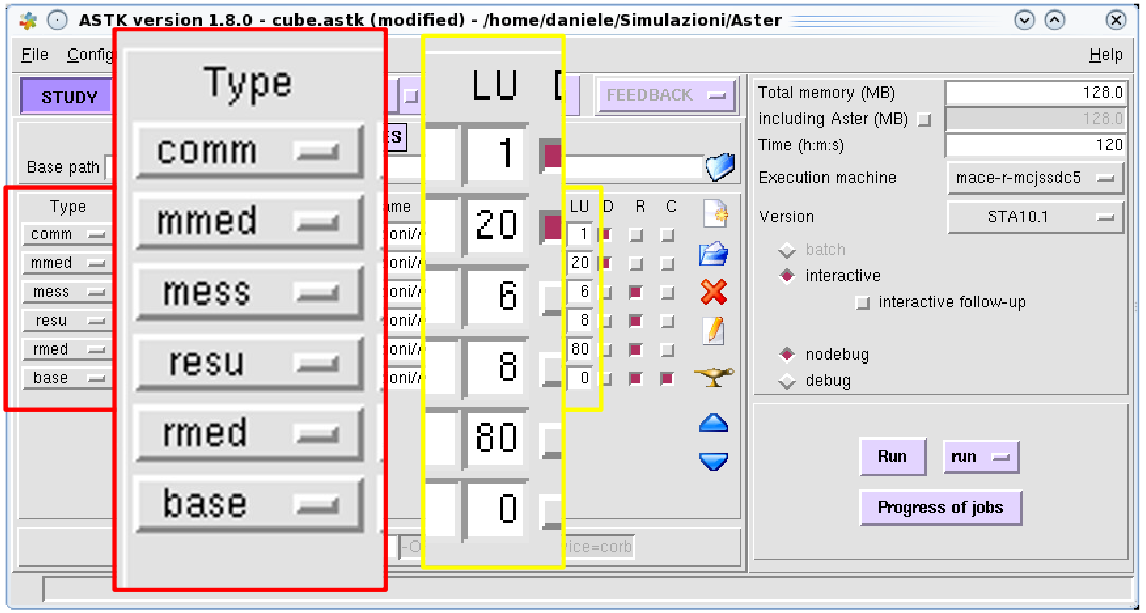
\includegraphics[width=5in]{numeroslogicos.png}
\caption{Números lógicos asigandos a los tipos de archivos}
\label{fig5}
\end{figure}

Si en número lógico no es dado como parámetro del comando, el volor por defecto 
utilizado es uno. En el siguiente ejemplo

\begin{verbatim}
 MAIL = LIRE_MAILLAGE(FORMAT='MED',);
\end{verbatim}

En el código anterior el comando LIRE\_MAILLAGE leerá el archivo asociado a valor 
lógico por defecto para los archivos de mallas con formato MED (rmed).. No es necesario
conocer cual es el valor por defecto de los números lógicos si estos no han
sido modificados manualmente en ASTK. Al contrario, si se cambiaron los
valores lógicos por defecto en ASTK, se debe proporcionar estos nuevos valores a el
comando a través de la palabra clave \textbf{UNITE}. De tal manera que si, por ejemplo,
al tipo de archivo mmed se le cambió el número lógico a 21 y se desea leer este
archivo, el comando quedaría:

\begin{verbatim}
 MAIL = LIRE_MAILLAGE(FORMAT='MED',UNITE=21,);
\end{verbatim}

\subsection{Comando AFFE\_MODELE}

Este comando permite asignar un modelo físico particular y tipo de elemento 
a una malla. Un modelo FE es creado. Primero debe seleccionarse la malla con el
 comando MAILLAGE. 


\begin{verbatim}
 MODE = AFFE_MODELE(MAILLAGE= MAIL, AFFE=_F(TOUT='OUI',
                    PHENOMENE='MECANIQUE', MODELISATION='3D',),);
\end{verbatim}

La palabra compuesta AFFE permite especificar los fenomenos
físicos y tipos de elementos para ser asignados a una parte o a toda la mesh:

\begin{itemize}
 \item \verb*|TOUT='OUI'| significa \verb*|WHOLE_MESH='YES'|
 \item \verb*|PHENOMENE='MECANIQUE'| especifica que se va a modelar fenómenos
        mecánicos (no térmicos ni acústicos)
 \item \verb*|MODELISATION='3D'| especifica que usaremos elementos sólidos de 3D
       (y no, por ejemplo, elementos ladrillos 3D)
\end{itemize}

El grupo de palabras claves dentro de \verb*|_F(...)| puede se repetido para
definir todos los modelos. Por ejemplo,en el caso en el cual tanto los elementos 
solidos en 3D y los ladrillos en 3D estan presentes en la malla, el siguiente comando
puede se usado para asignar las propiedades de los elementos:

\begin{verbatim}
 mode = AFFE_MODELE(MAILLAGE=MAIL, AFFE=(_F(GROUP_MA='solid',
                   PHENOMENE='MECANIQUE',
                   MODELISATION='3D',),
                  _F(GROUP_MA='beam',
                     PHENOMENE='MECANIQUE',
                     MODELISATION='POU_D_E',),),)
\end{verbatim}
\textit{Solid} y \textit{beam} son dos grupos de elementos (\verb*|GROUP_MA|) definido 
dentro de la malla MAIL (con la ayuda de Salome).

\subsection{Comando AFFE\_MATERIAU}

Este comando permite asignar un material a elementos de una malla. La sintaxis es 
muy simular a las discutidas anteriormente. El material debe ser definido anteriormente
usando el comando DEFI\_MATERIAU. El concepto creado por el comando es un campo
material, una entidad poco usual en los solvers de elementos finitos. Supongamos 
que se definieron dos materiales por ejemplo \textit{steel} y \textit{alu} de las páginas
anteriores. Y supongamos que se han definido dos grupos de elementos en la malla, cada 
una conteniendo elementos del mismo material:

\begin{itemize}
 \item \textbf{ELsteel} que contiene los elementos para acero
 \item \textbf{ELalu} contiene los elementos para aluminio
\end{itemize}
La unión de los dos grupos cubre los elementos de la malla, esto es cada elemento
de la malla pertenece a alguno de los dos grupos.

La asignación de los materiales puede realizarse de la siguiente manera:

\begin{verbatim}
 mate = AFFE_MATERIAU(MAILLAGE=MAIL, 
                      AFFE=(_F(GROUP_MA='ELsteel', MATER=steel,
                            _F(GRUOP_MA='ELalu', MATER=alu,),),)
\end{verbatim}

Otra solución puede ser usar la regla superposición:

\begin{itemize}
 \item Si mas de una propiedad es asignada a la misma entidad, solamente la
 última es considerada.
 \item En otras palabras, si cada asignación sobreescribe a la previa.
\end{itemize}

La versión de sobreescritura de la asignación es la siguiente:

\begin{verbatim}
 mate = AFFE_MATERIAU(MAILLAGE=MAIL, 
                      AFFE=(_F(TOUT='OUI', MATER=steel,
                            _F(GRUOP_MA='ELalu', MATER=alu,),),)
\end{verbatim}

En el comando anterior sucede los siguiente:

\begin{itemize}
 \item Primero, el material \textit{steel} es asignado a todos los elementos de 
la malla MAIL.
 \item Entonces, el material \textit{alu} es asignado solamente a los elementos
en el grupo \textbf{ELalu}
 \item El material \textit{steel} asignado previamente a estos elementos
(\textbf{ELalu}) es sobre escrito debido a la segunda asignación
\end{itemize}

El uso de la regla de sobreescritura puede ser realmente efctivo en muchas 
situaciones. Aún es este ejemplo simple, la ventaja será:

\begin{itemize}
 \item Solamente un grupo de elementos (\textbf{ELalu}) puede ser definido
y mantenido en la malla.
 \item Una material es asigando a todos los elementos de la malla. No hay
riesgo que uno o mas elementos no tengan material asignado porque esten fuera de los
dos grupos definido (\textbf{ELsteel} y \textbf{ELalu}) consecuencia de un error en
la creación de los grupos. 
\end{itemize}

\subsection{Comando AFFE\_CHAR\_MECA}

Este comando permite asignar cargas mecánicas, condiciones de frontera y restricciones
cinemáticas a el modelo por elementos finitos. Las opciones:
\begin{itemize}
 \item DDL\_IMPO asiga un valor a uno o mas grados de libertad de un nodo.
 \item PRES\_REP aplica una presión un dominio 2D/3D.
\end{itemize}

Un ejemplo de código es:

\begin{verbatim}
 CHAR = AFFE_CHAR_MECA(MODELE = MODE, 
                       DDL_IMPO = _F(GROUP_MA='Down',
                                     DX=0.0,
                                     DY=0.0,
                                     DZ=0.0,),
                       PRES_REP = _F(GROUP_MA='UP',
                                     PRES=100.0,),);
\end{verbatim}

\subsection{Comando MECA\_STATIQUE}

Permite en ensamblaje del conjunto discreto de ecuacione por elementos finitos 
y resolverlas usando un modelo lineal estático Mecánico. Al contrario de otros solvers 
por elementos finitos, en este punto el usuario debe especificar el modelo, 
los materiales y las cargas que será aplicadas y usadas en el ensamble.

Esto significa que no todos los materiales definidos, cargas, condiciones de 
frontera y modelos serán usados durante el ensamblado del modelo por elementos
finitos que será resuelto.

El comando MECA\_STATIQUE no puede ser usado si hay presente no linealidades (ya sean 
geométricas y/o en el comportamiento del material). Si es el caso debe usarse 
el comando STAT\_NON\_LINE. Similarmente, otros comandos deben usarse en el caso de 
una simulación dinámica (DYNA\_NON\_LINE, DYNA\_LINE\_TRAN\/DYNA\_LINE\_MODAL, 
DYNA\_LINE\_HARM...). Otros comandos pueden ser usados en el caso de simulación térmica
 (THER\_LINEAIRE, THER\_NON\_LINE, THERM\_NON\_LINE\_MO)


\begin{verbatim}
 RESU=MECA_STATIQUE(MODELE=MODE,
                   CHAM_MATER=MATE,
                   EXCIT=_F(CHARGE=CHAR,),);
\end{verbatim} 

El concepto creado por el solver (RESU) contiene los resultados del análisis: El
campo de desplazamiento del modelo. Esto es un campo nodal.

\subsection{Comando CALC\_ELEM}

Este comando permite calcular uno o mas campos asociados a un elemento, como por 
ejemplo estres, compresión etc. Los campos a ser calculados son especificados 
con la palabra clave OPTION. Los calculos son realizados iniciando con el concepto
RESU (RESULTAT=RESU) el cual contiene los resultados de la simulación (solamente 
desplazamientos nodales).
\begin{verbatim}
 RESU=CALC_ELEM(reuse=RESU,
                MODELE=MODE,
                CHAM_MATER=MATE,
                RESULTAT=RESU,
                OPTION=('SIGM_ELNO_DEPL', ' EQUI_ELNO_SIGM',),
                EXCIT=_F(CHARGE=CHAR,),);
\end{verbatim} 
El concepto creado por el comando es RESU. Este ya existia porque fue creado por el
comando MECA\_STATIQUE.

El objetivo del comando es enriqueser el concepto: Algunos campos nuevos son 
adicionados (estos son específicamente usados por la palabra clave OPTION):
\begin{itemize}
 \item El concepto producido por el comando no debe 
 \item Debemos declarar nuestro objetivo usando la palabra \textbf{reuse}
 \item De lo contrario, debe cambiar el nombre del concepto a la izquierda del
signo igual
\end{itemize}

\begin{verbatim}
 RESU=CALC_ELEM(reuse=RESU,
                RESULTAT=RESU,
                OPTION=('SIGM_ELNO_DEPL', ' EQUI_ELNO_SIGM',),
                ,);
\end{verbatim} 

Los calculos son realizados empezando desde un concepto de tipo ``result'' (RESULTAT=RESU).
Este tipo de concepto contiene toda la información del modelo ademas de los
campos de desplazamiento nodales (el cual es efectivamente el resultado):

\begin{itemize}
 \item Las palabras claves MODELE, CHAM\_MATER y EXCIT son por lo tanto inútiles
en este caso y deben ser ignoradas.
 \item Estas palabras claves deben ser usadas solamente si la información pasada
a través de ellos no esta disponible en el concepto proporcionado por RESULTAT
\end{itemize}

\begin{figure}
\centering
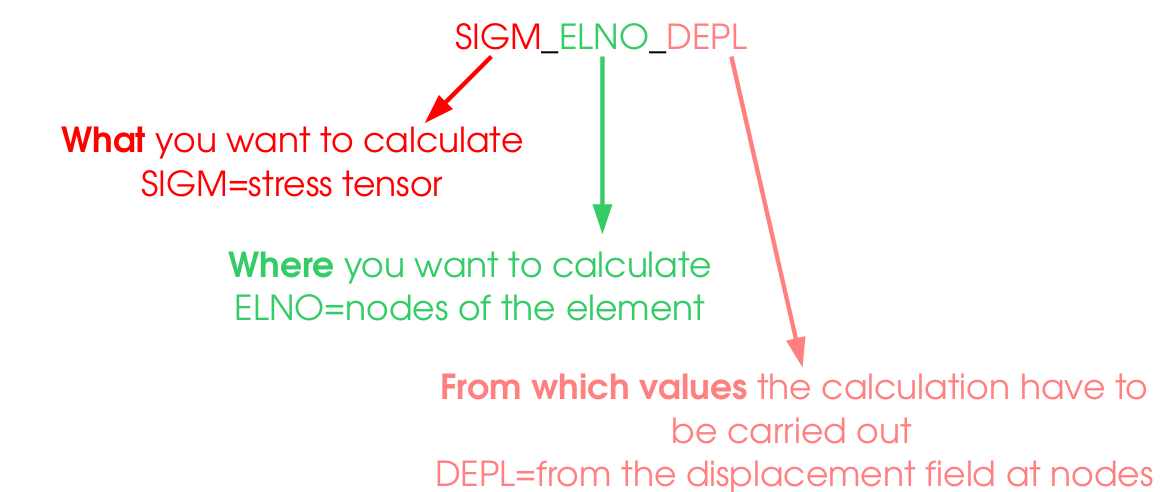
\includegraphics[width=5in]{significado.png}
\caption{Significado de los campos en la palabra OPTION}
\label{fig6}
\end{figure}
En la figura \ref{fig6} se muestra el significado de las tres partes que forman 
las opciones del comando OPTION.
\begin{figure}
\centering
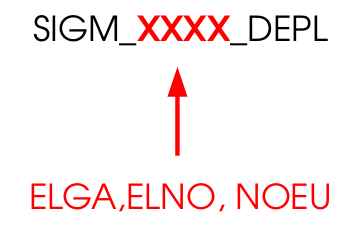
\includegraphics[width=3in]{opciones.png}
\caption{Opciones para la aplicación de los análisis}
\label{fig7}
\end{figure}

En la figura \ref{fig7} se muestran las opciones para el comando OPTION sobre
las cuales se aplicará el análisis:

\begin{itemize}
 \item ELGA (\textbf{ELement GAuss}): Los calculos deben hacerse en los puntos Gauss
de los elementos.
 \item ELNO (\textbf{ELement NOde}): Los calculos deben hacerse en los nodos de cada
elemento, considerado separado de los elementos vecinos. Mas de un valor es calculado
para cada nodo, un valor para cada elemento compartiendo ese nodo.
 \item NOEU (\textbf{node}): Los calculos son hechos en cada nodo. Un valor principal
de los valores que vienen de cada elemento que comparte en nodo es calculado.
\end{itemize}

La diferencia entre los valores calculados en ELNO y los calculados en NOEU son debido
a la discretización FE.

\subsection{Comando CALC\_NO}
Este comando permite calcular uno o mas campos asociados a un nodo, este comando
trabaja como CALC\_ELEM. Se pueden calcular campos nodales: Fuerzas de reacción, fuerzas
nodales y todos los campos de tipo xxxx\_NOEU\_xxxx. El campo xxxx\_NOEU\_xxxx pueden
ser calculado solamente si el campo correspondiente ELNO existe en el concepto 
que nos da RESULTAT.

\begin{figure}
\centering
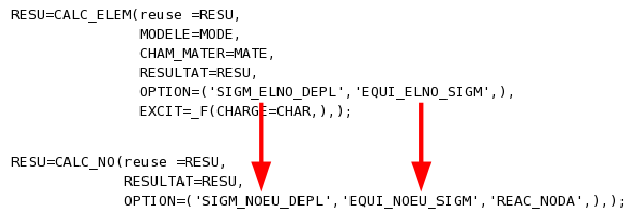
\includegraphics[width=5in]{CALC_NO.png}
\caption{Como usar el comando CALC\_NO}
\label{fig8}
\end{figure}
En la figura \ref{fig8} se muestran la correspondencia que debe haber entre el comando
SIGM\_NOEU\_DEPL y EQUI\_NOEU\_SIGM con los comandos xxxx\_ELNO\_xxxx, es decir, 
si se  intenta calcular xxxx\_NOEU\_xxxx sin calcular primero  xxxx\_ELNO\_xxxx 
CODE ASTER indicará una advertencia y NO realizará los cálculos. 

\subsection{Comando IMPR\_RESU}

Este comando permite imprimir los resultados en uno o más archivos de salida. El 
formato es escogido por la palabra clave FORMAT. Si no se especifica ningun campo
(NOM\_CHAM), todos los campos dentro del resultado (\verb|RESULTAT=RESU|) serán escritos
en el archivo de salida. Es importante mencionar que ningún concepto es creado
con este comando. Muchos formatos son soportados para salida:I-DEAS, MED, CASTEM, GMSH, RESULTAT. Si \verb|FORMAT='RESULTAT'| es usado, la salida se escribira en un
archivo de texto en una o más tablas. Por ejemplo


\begin{verbatim}
 IMPR_RESU(FORMAT='RESULTAT',
           RESU=_F(MAILLAGE=MAIL,
           RESULTAT=RESU,
           NOM_CHAM=('SIGM_NOEU_DEPL', 'EQUI_NOEU_SIGM', 'DEPL',),),);
\end{verbatim} 

\subsection{Comando FIN}

Todos los archivos de comandos deben terminar con este comando e indida en fin 
del archivo de comandos.

\backmatter
\end{document}
